\section{Durchführung / Implementierung}\label{sec:durchfuehrung-implementierung}

Die Entwicklung des Projekts lässt sich grob ich zwei Phasen aufteilen.
Die erste Phase ist die Planungsphase, in welcher die Anforderungen an das Projekt definiert und die Architektur der Anwendung festgelegt wurde.
Die Resultate aus dieser Phase wurden in den vorherigen Kapiteln beschrieben.
Beendet wurde diese Phase mit der ersten Präsentation des Projekts, in welcher die Projektidee vorgestellt wurde.
Die zweite Phase ist die Durchführungsphase, in welcher die Anwendung umgesetzt wurde und welche im diesem Kapitel beschrieben wird.
Gestartet hat diese Phase direkt nach dem Ende der ersten Phase, nach welcher die Erlaubnis zur Durchführung des Projekts erteilt wurde.
Hierbei wurden die Aufgaben basierend auf dem Organigramm verteilt.
Während die Verantwortlichen für die Datenbank und das Backend sich des Öfteren Abstimmen mussten, konnte das Frontend-Team weitestgehend unabhängig arbeiten.
Jedes Teammitglied hat sich selbstständig in die Thematiken eingearbeitet, die für die Umsetzung ihres Verantwortungsbereichs nötig waren.

Der übliche Ablauf während der Durchführungsphase war es, dass sich das Team einmal in der Woche zusammengesetzt hat, um den aktuellen Stand der Projektbausteine zu besprechen.
Hierbei wurde abgesprochen, welche Aufgaben bis zum nächsten Treffen erledigt werden sollten.
Mussten Abschnitte aus einzelnen Bereichen zusammengeführt werden, wurde dies in einem separaten Meeting besprochen, woran nur die verantwortlichen Teammitglieder teilgenommen haben.
Die Aufgaben wurden mit YouTrack verwaltet, wodurch immer ein klares Verständnis über die Aufgabenverteilung herrschte.
Das Dashboard wurde während den Team Meetings basierend auf dem Stand und der Verteilung aktualisiert.
Die Aufgaben wurden in Open, In Progress, To Be Reviewed und Done unterteilt.
Ein Einblick in die YouTrack Aufgabenverwaltung ist in Abbildung~\ref{fig:youtrack_screenshot_agile_board} zu sehen.

\begin{figure}[h]
    \centering
    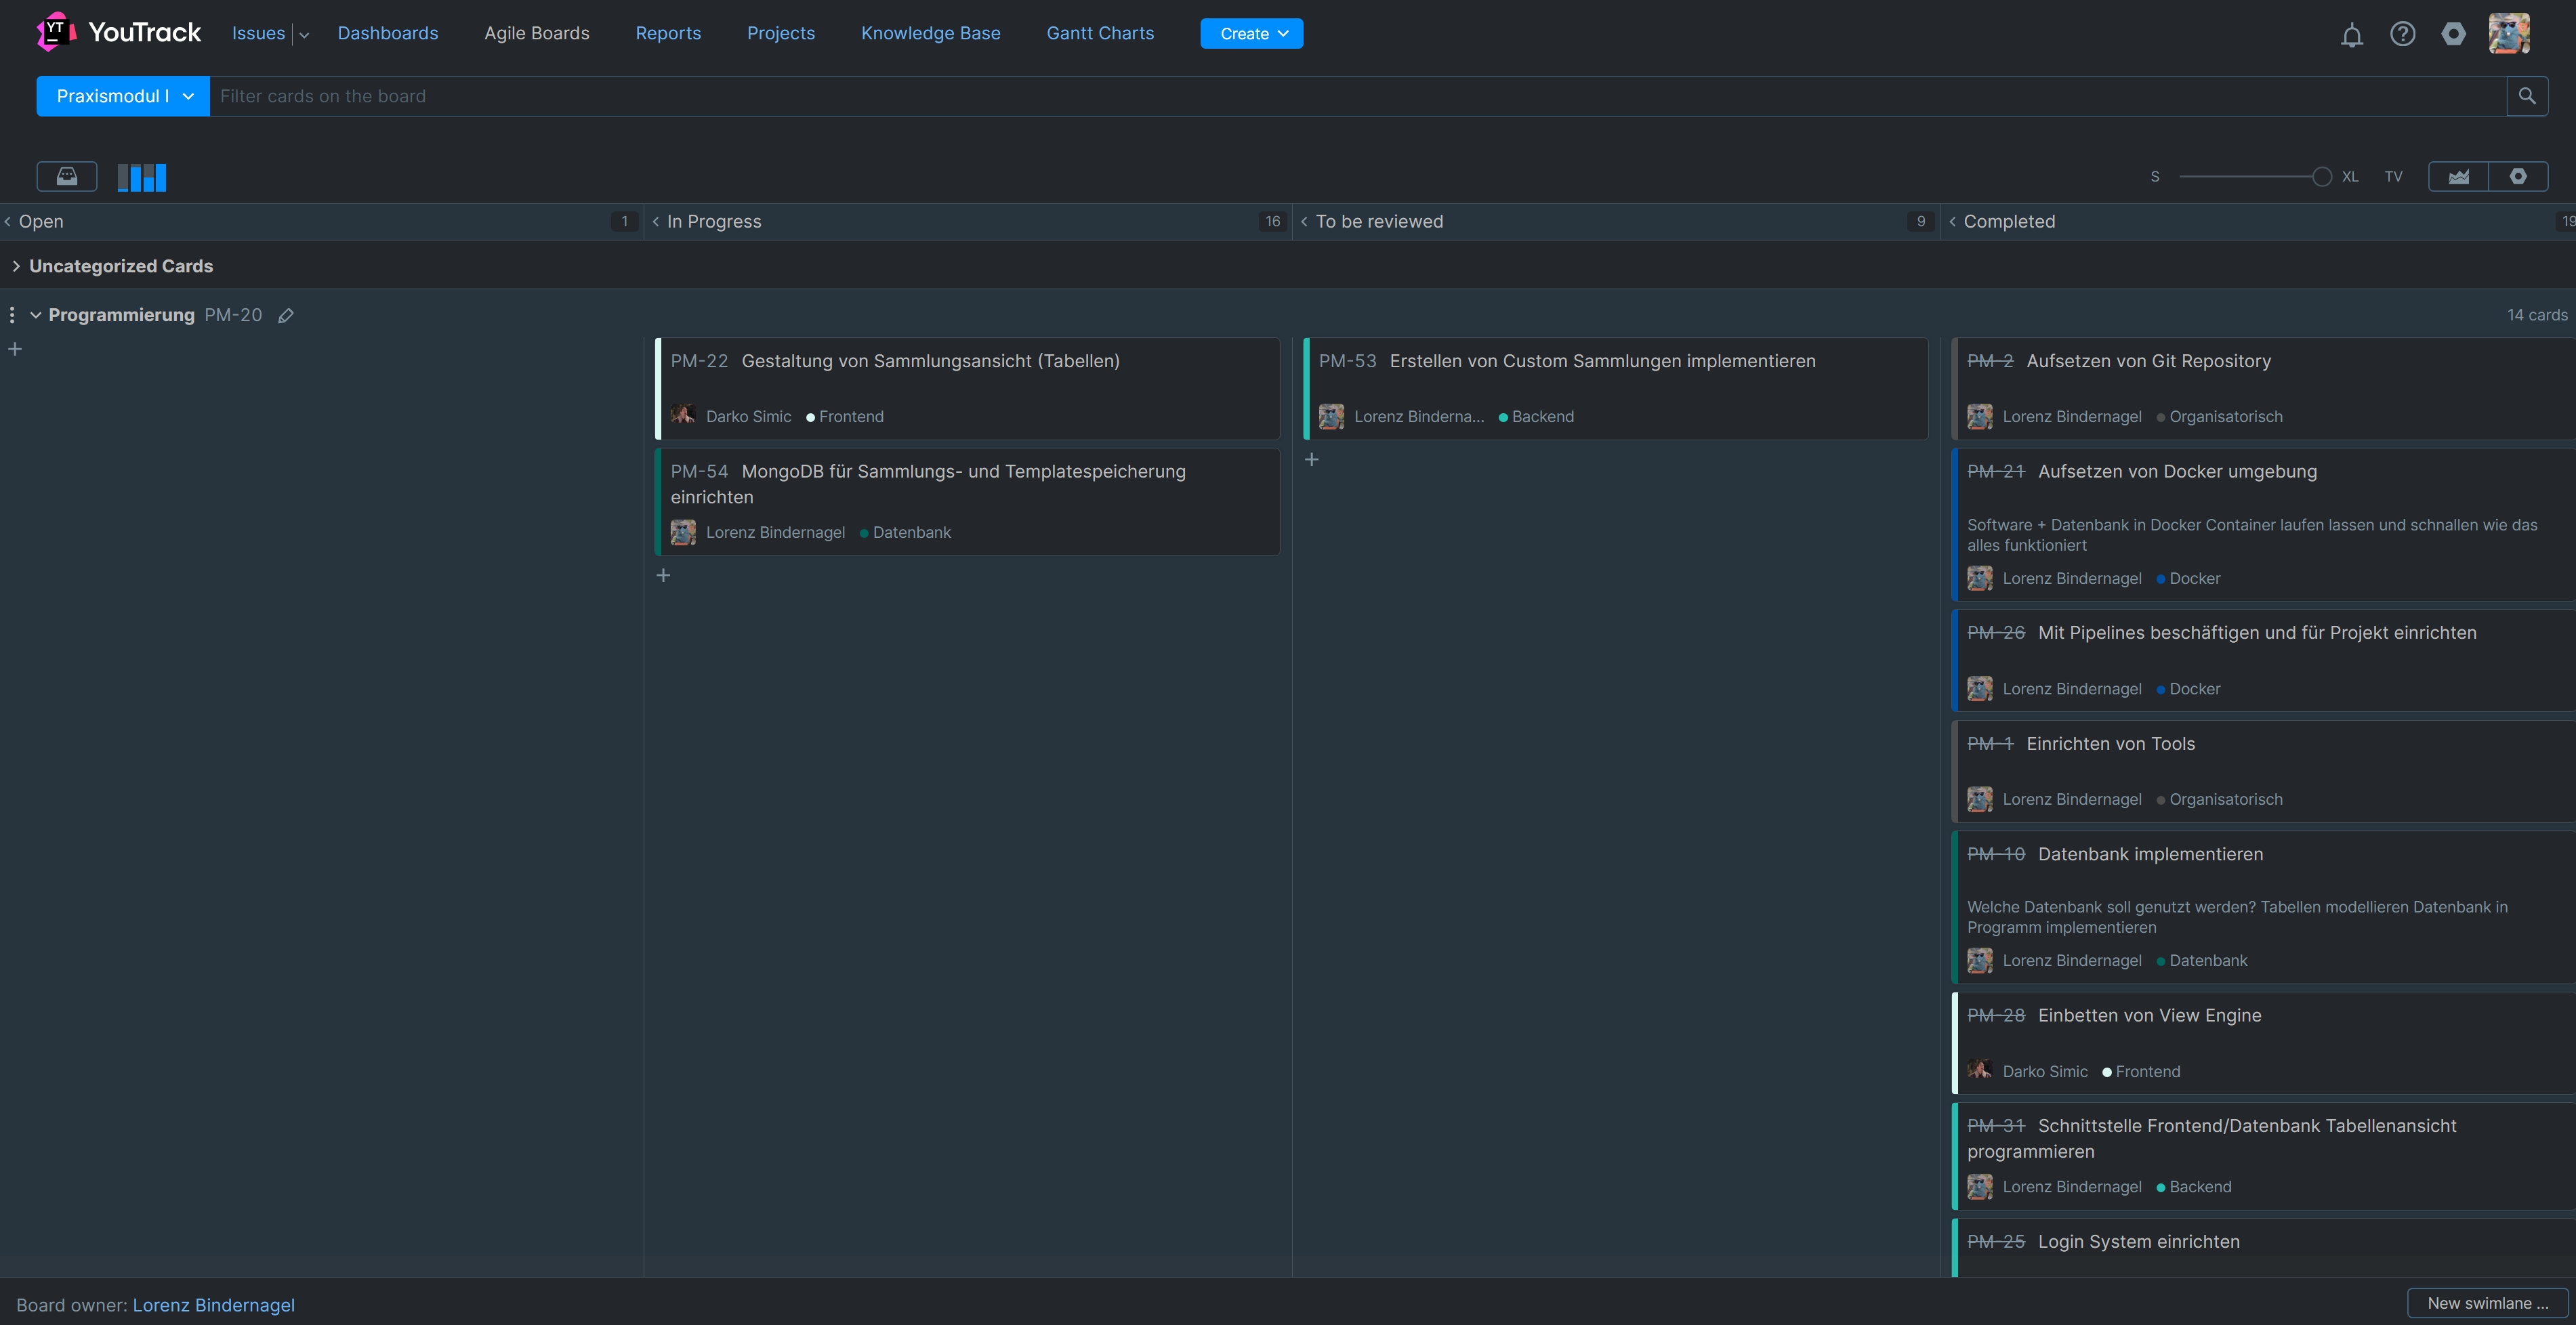
\includegraphics[width=1\textwidth]{youtrack_screenshot_agile_board}
    \caption{Screenshot des Agile Dashboards in YouTrack}
    \label{fig:youtrack_screenshot_agile_board}
\end{figure}

\subsection{Entwicklung des Webfrontends}\label{subsec:entwicklung-des-webfrontends}
Die Entwicklung des Webfrontends konzentrierte sich auf die Erstellung einer benutzerfreundlichen Oberfläche und alle nötigen Grundfunktionen und Strukturen.
Mithilfe von HTML, CSS und EJS wurde eine schlichte Webseite gestaltet.

Das Herzstück der Webseite ist das Anlegen eigener Collections, welche dynamisch mit Daten aus der hinterlegten MongoDB Datenbank befüllt wird.
Die Datenbank wird dabei durch JavaScript und dessen Frameworks und Bibliotheken angesprochen, welche wiederum durch das Frontend angestoßen werden.
Für das Webfrontend wurde eine Express-Anwendung in Node.js erstellt, welche auf statische Dateien (CSS, JS, Bilder) aus dem Ordnerverzeichnis zugreift.
Die Verwendung von Node.js ermöglicht das Definieren von HTTP Routen mit JavaScript, um so durch die verschiedenen Seiten der Webseite navigieren zu können und serverseitige Funktionen aufzurufen.

EJS wurde als Template-Engine verwendet, um die Integration von JavaScript innerhalb von HTMLDokumenten zu ermöglichen und somit auch seine Sammlungen abrufen zu können.
Dies erlaubte eine flexible und dynamische Gestaltung der Webseite, insbesondere durch die Verwendung von EJS-Tags wie \grqq\textless{}\%=\%\textgreater{}\grqq{}, die es ermöglichte, serverseitige Variablen oder Ausdrücke direkt in die HTML-Struktur einzufügen.
In diesem Fall wurden die Collections aus der Datenbank abgerufen und über eine Schleife in der EJS-Vorlage gerendert und werden einmal in einer Übersicht angezeigt.
In dieser Übersicht hat man die Möglichkeit eine beliebig angelegte Collection anzuklicken um so diese anzuschauen oder auch zu bearbeiten.

\subsection{Entwicklung des Backends}\label{subsec:EntwicklungDesBackends}
Der erste Schritt bei der Backend entwicklung war es, einen geeigneten Startpunkt zu finden.
Hierbei wurde entschieden, dass zuerst eine Implementierung der Datenbankverbindung erfolgen sollte, da diese als Grundlage für die weitere Entwicklung dient.
Dies wurde mit der Bibliothek mysql2 realisiert, welche eine erweiterte Funktionalität gegenüber der Standardbibliothek bietet und diverse Probleme behebt.
Diese implementierung war erst möglich, nachdem die Grundstruktur der Datenbank aufgesetzt wurde.
Einen Einblick in den Code gibt Listing\ref{lst:connecttomysql}.

\lstinputlisting[language=JavaScript,label={lst:connecttomysql}]{../server/dbConnections/connectToMYSQL.js}

Als Nächstes wurde sich dazu entschieden, ein einfaches Sign Up und Login System zu programmieren.
Hierbei wurde auf die Bibliothek bcrypt zurückgegriffen, welche das Hashen von Passwörtern erleichtert.
Die SQL queries, die hier genutzt werden, wurden ebenfalls mit der mysql2 Bibliothek realisiert.
Die einzigen Nutzerdaten, die hierbei gespeichert werden, sind der Username, die E-Mail und das Passwort.
Beim Login wurde darauf geachtet, das Nutzer Username und E-Mail benutzen können, um sich einzuloggen.
Ein Einblick in den Code gibt Listing\ref{lst:login}.

\lstinputlisting[languange=JavaScript,label={lst:login}]{../server/authentication/loginHandler.js}

Nun stellte sich die Frage, wie es möglich ist, dass Nutzer nur auf ihre eigenen Sammlungen zugreifen können.
Beim Recherchieren sind wir auf das Konzept von Sessions gestoßen und wollten diese ausprobieren.
Die erste Anwendung fanden Sessions im Speichern des Usernamens in einer Session Variable, nachdem der User sich angemeldet hat.
Der nächste Schritt war es, die Sammlungen eines Nutzers basierend auf dem Usernamen aus der Datenbank zu laden.
Zuvor muss jedoch erstmal eine Funktion implementiert werden, mit der Sammlungen angelegt werden können.
Hierzu muss zuerst die Datenbank implementiert werden, in welcher die Sammlungen gespeichert werden.
Als Datenbank für die Sammlungen wurde sich für MongoDB entschieden, welches im Kapitel~\ref{subsec:entwicklung-der-datenbank-und-datenstruktur} genauer erläutert wird.

Nur das Anlegen von Sammlungen reicht natürlich nicht, weshalb weitere Funktionen im Backend implementiert wurden, die diverse grundlegende Funktionen ermöglichen.
Hierzu zählen das Löschen von Sammlungen, das Hinzufügen von Items zu Sammlungen und das Löschen von Items aus Sammlungen.
Außerdem wurde eine separate Funktion implementiert, die das Erstellen einer Sammlung direkt von einem Template aus ermöglicht.
Das Hinzufügen von Daten in eine existierende Sammlung wird mit dem folgenden Code ermöglicht:

\lstinputlisting[language=JavaScript, label={lst:addCollectionEntry}]{../server/collections/addCollectionEntry.js}

Während der Entwicklung des Backends kam es jedoch auch des Öfteren zu Herausforderungen.
Eine dieser Stellen war der Umgang mit Docker Containern.
Ein gewisses Grundverständnis war vorhanden, doch an praktischer Erfahrung fehlte es dem Team.
Zwar was das Hochfahren einer Datenbank in einem Container schnell erreicht, doch ein Verständnis für Datenpersistenz und Volumes zu entwickeln, benötigte seine Zeit.
Auch im späteren Verlauf des Projekts, als es darum ging alle Applikationskomponenten in einer Docker-Compose Datei zusammenzuführen, stellte sich als Herausforderung heraus.
Wie sich Dockerfiles in dem ganzen System einordnen und wo sie genutzt werden, war ebenfalls neu für das Team.
Allgemein hat das Einfinden in Docker dem Team mehr Zeit als erwartet abverlangt.
Am Ende sah die Docker-Compose Datei wie in Listing~\ref{lst:docker-compose} aus.
Die Images für die beiden Datenbanken sind selbst erstellt, auf der Grundlage von den offiziellen MongoDB und MySQL Images.
Diese beinhalten beispieleinträge für diverse Sammlungen verschiedener Nutzer, bereits angelegte Testnutzer und die Datenbankstruktur inklusive der Templates für die Sammlungen.

\lstinputlisting[language=docker-compose, label={lst:docker-compose}]{../docker-compose.yaml}

Eine weitere Herausforderung war das Einfinden in die verschiedenen Bibliotheken, die bei Webentwicklung mit JavaScript genutzt werden.
Zwar wurde in der Planung bereits einige Bibliotheken festgelegt, die genutzt werden sollten, doch während der Entwicklung kamen einige neue hinzu.
Ein Beispiel hierfür ist die Bibliothek express-session, die für das Session-Management genutzt wird.
Da zur Planung noch kein detailliertes Verständnis darüber vorhanden war, welche Komponenten bei der Entwicklung einer solchen Anwendung benötigt werden, wurden Thematiken wie Session Management erst während der Entwicklung entdeckt.
Hierdurch kam es an einigen Stellen zu steilen, jedoch unvermeidbaren Lernkurven, die jedoch auch entsprechenden zeitlichen Aufwand mit sich gebracht haben.

Da das Team zuvor noch nie eine Webanwendung entwickelt hat, fehlte es an Verständnis, wie viel Komponenten Teil einer solchen Anwendung sind.
So kam es, dass während der Entwicklung immer wieder neue Komponenten entdeckt wurden, die in der Planung nicht berücksichtigt wurden.
Ein konkretes Beispiel hierfür ist das Session-Management.

\subsection{Entwicklung der Datenbank und Datenstruktur}\label{subsec:entwicklung-der-datenbank-und-datenstruktur}

Bei der Einrichtung der Datenbank stellt sich als erste Hürde der Umgang mit Docker Container heraus.
Zwar waren grundlegende Kenntnisse über Docker vorhanden, doch eine Datenbank praktisch in einem Container hochzufahren und diese dann mit dem Code und der Programmierumgebung zu verknüpfen, war eine neue Herausforderung.
Wie in der Planung entschieden, sollen zwei Datenbanken genutzt werden - eine MySQL Datenbank für strukturierte Daten und eine MongoDB Datenbank für unstrukturierte Daten.
Im ersten Schritt wurde die MySQL Datenbank aufgesetzt und mit Tabellen für Nutzerdaten und den drei Pre-Sets für Sammlungen befüllt.
Die Nutzerdaten beinhalten Username, E-Mail und Passwort.
Da diese Tabelle eine feste Form besitzt, wurde sich für eine relationale Datenbank entschieden.
Die Struktur der MySQL Datenbank ist in Abbildung~\ref{fig:mysql_structure} zu sehen.

\begin{figure}[h]
    \centering
    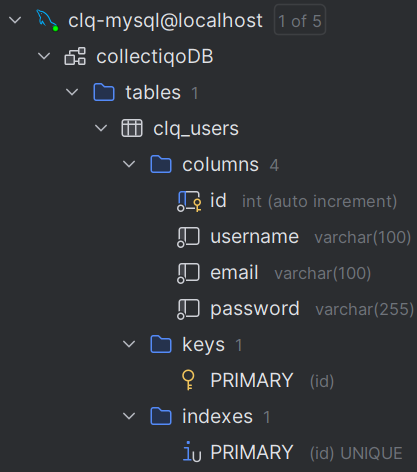
\includegraphics[width=0.4\textwidth]{mysql_structure}
    \caption{Struktur der MySQL Datenbank}
    \label{fig:mysql_structure}
\end{figure}

Als Datenbank für die Sammlungen und die Vorlagen wurde sich für eine MongoDB Datenbank entschieden.
Dies liegt daran, dass MongoDB eine dokumentenorientierte Datenbank ist, die sich gut für die Speicherung von unstrukturierten Daten eignet.
Die Daten der Sammlungen sind unstrukturiert, da sie sich je nach Thema unterscheiden, da jede Sammlung andere Spalten besitzt.
Dasselbe gilt für die Vorlagen, die zum Erstellen von Sammlungen genutzt werden können.
Dies ist das erste Mal, dass das Team mit einer dokumentenorientierten Datenbank arbeitet, daher musste erstmal ein Verständnis über den Aufbau einer solchen Datenbank geschaffen werden.
Zunächst wurde versucht vergleiche mit einer SQL Datenbank herzustellen, wobei schnell auffiel, dass Konzepte wie Schemata hier Collections sind.
Für dieses Projekt wurden zwei verschiedene Collections angelegt, eine für die Vorlagen, die zum Erstellen eigener Sammlungen genutzt werden können und eine für die Sammlungen selbst.
Die Struktur der MongoDB Datenbank ist in Abbildung~\ref{fig:mongodb_structure} zu sehen.

\begin{figure}[h]
    \centering
    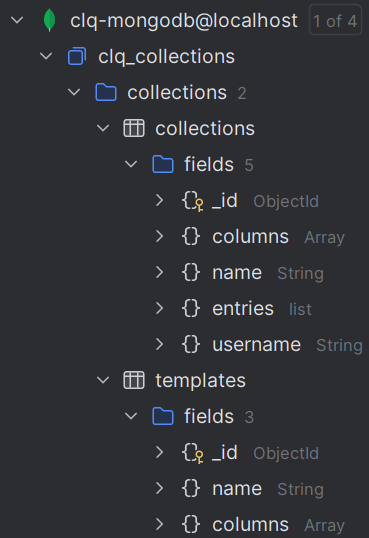
\includegraphics[width=0.4\textwidth]{mongodb_structure}
    \caption{Struktur der MongoDB Datenbank}
    \label{fig:mongodb_structure}
\end{figure}

Die Daten innerhalb der Collection für die Sammlungen sieht wie in Abbildung~\ref{fig:mongodb_collections} aus.
Die Sammlung für Videospiele wurde hierbei anhand einer Vorlage aus dem Vorlagenkatalog erstellt.

\begin{figure}[h]
    \centering
    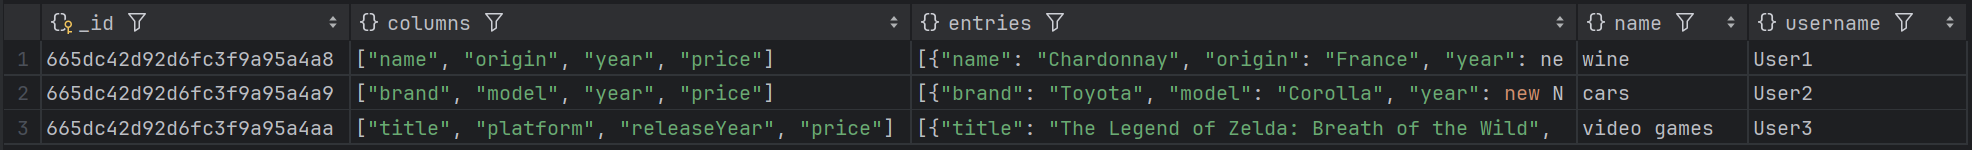
\includegraphics[width=1\textwidth]{mongodb_collections}
    \caption{Daten innerhalb der MongoDB Collection}
    \label{fig:mongodb_collections}
\end{figure}

Einzelne Einträge innerhalb der Collections werden wie in Abbildung~\ref(fig:mongodb_collections_entries) strukturiert.
Die Spalten sind exemplarisch für eine Autosammlung und ändern sich je nach Thematik.

\begin{figure}[h]
    \centering
    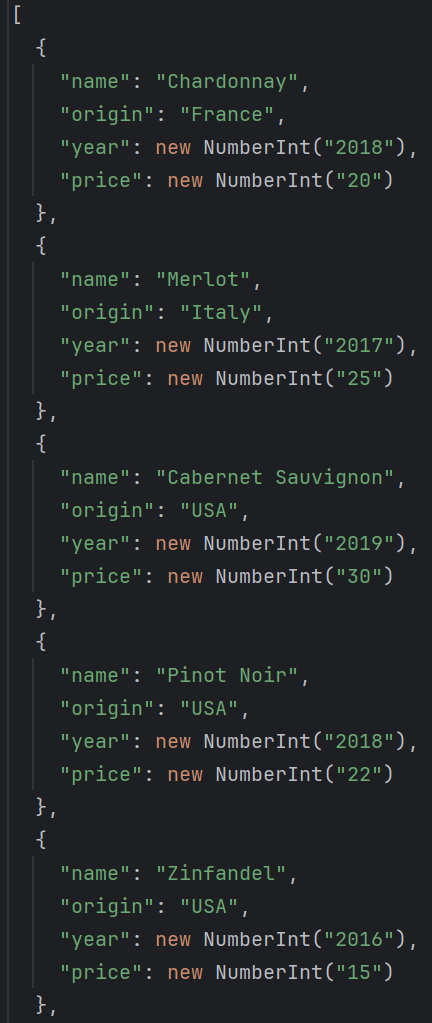
\includegraphics[width=0.4\textwidth]{mongodb_collections_entries}
    \caption{Einträge innerhalb einer Sammlung}
    \label{fig:mongodb_collections_entries}
\end{figure}

Die Vorlagen für die Sammlungen sind in Abbildung~\ref{fig:mongodb_templates} zu sehen.
Aktuell sind diese festgelegt, ohne Option diese zu verändern oder neue hinzuzufügen und sie sind gültig für alle User der Website.
In späteren Versionen soll jedoch das Anlegen von eigenen Vorlagen möglich sein, welche dann auch einzelnen Nutzern zugewiesen werden.
Bringt man einen Community-Aspekt mit ein, so könnte es in zukunft möglich sein, diese Vorlagen untereinander zu teilen.

\begin{figure}[h]
    \centering
    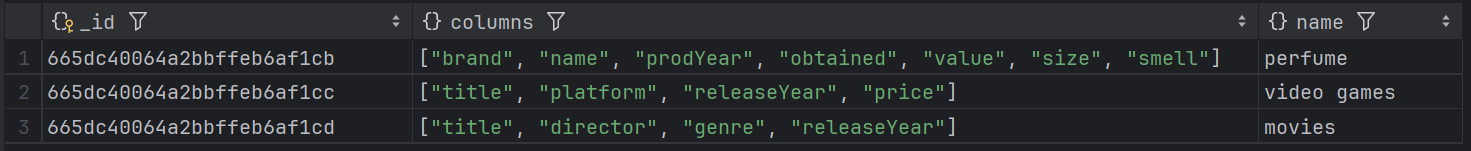
\includegraphics[width=1\textwidth]{mongodb_templates}
    \caption{Daten innerhalb der MongoDB Collection für die Vorlagen}
    \label{fig:mongodb_templates}
\end{figure}

Das Integrieren der Datenbank in der Programmierumgebung war schnell erledigt, da dies analog zu der MySQL Datenbankverbindung erfolgt ist.
Das Auslesen und schreiben von Daten in die Datenbank war dank der MongoDB Bibliothek einfach erledigt.
Funktionen für die Verbindung mit der Datenbank wurden in einer separaten Datei ausgelagert.

Die Herausforderungen, die beim Einrichten des Datenbanksystems entstanden sind, teilen sich in zwei Punkte auf.
Der erste Punkt hängt damit zusammen, dass das Einrichten der Datenbanken gleichzeitig die erste praktische Nutzung von Docker Containern war.
Somit musste erstmal ein Verständnis dafür entwickelt werden, wie vom Hostsystem auf die Container zugegriffen werden kann und wie Daten persistiert werden.
Da die Datenbanken vorgefertigten Inhalt benötigten, wie bspw.\ die Templates für die Sammlungen in der MongoDB oder das Datenbankschema für User in der MySQL Datenbank, musste sich angeeignet werden, wie Docker Images erstellt werden können.
Darüber hinaus musste recherchiert werden, wie man solche Images hosten kann, sodass jeder beim Starten der Docker Compose Datei die Datenbanken mit den nötigen Inhalten erhält.
Die Herausforderungen ähneln somit denen, die bereits bei der Entwicklung des Backends aufgetreten sind.

\subsection{Verbinden des Frontends und Backends}\label{subsec:verbinden-des-frontends-und-backends}

Der erste Schritt beim Verbinden von Front- und Backend war es, das Login und Sign Up System zu verbinden.
Nach anfänglichen Problemen mit Umgebungsvariablen, die nicht korrekt geladen wurden aufgrund einer Umstrukturierung der Projektdokumentation, war der Prozess relativ einfach.
Es musste recherchiert werden, wie die Backendfunktionen seitens des Frontends aufgerufen werden, welches durch HTTP Requests realisiert wurde, die die Routen in der app.js ansprechen.
Da sich die Entwickler des Front- und Backends während der getrennten Entwicklung regelmäßig abgesprochen haben, konnten die Funktionen schnell miteinander verbunden werden.

\subsection{Implementieren von Tests}\label{subsec:implementieren-von-tests}

Um Teile des Backends zu testen, bevor diese mit dem Frontend verbunden werden konnten, wurde versucht Unit-Tests zu schreiben.
Dieser Prozess stellte sich als komplizierter heraus als gedacht, da das Team zuvor noch nie mit Tests für JavaScript gearbeitet hat.
So konnten zwar einfache Unit-Tests für das Login System geschrieben werden, jedoch Integrationstests, in welchen die Datenbank angesprochen wird, stellten sich als schwierig heraus.
Ein exemplarischer Test für das Login System ist in Listing~\ref{lst:loginTest} zu sehen.


\lstinputlisting[language=JavaScript, firstline=15, lastline=32, label={lst:loginTest}]{../test/loginHandler.test.js}


Auch gab es Probleme damit, eine Datei für Umgebungsvariablen für Testdatenbanken korrekt in die Tests mit einzubinden.
Erst nach längerer Recherche stellte sich heraus, dass Umgebungsvariablen für jest Tests in einer separaten Config Datei definiert werden müssen und nicht wie die normale .env Datei in den Code eingebunden werden konnte.
Auch mit den Mock Funktionen von jest musste sich erst eingearbeitet werden.
An dieser Stelle wurde sich dazu entschieden, die implementierung von Tests für alle Backend Funktionen abzubrechen, da der Aufwand zu groß war und die Zeit zu knapp.
Der zeitliche Aufwand für das Einrichten der automatisierten Tests war zu hoch, vor allem im Vergleich zu dem zeitlichen Aufwand den ein manueller Test benötigt hätte.
Manuelle Tests wurden durchgeführt, als das Backend mit dem Frontend verbunden war.
Ein Nachteil, der dadurch entstanden ist, ist dass Funktionen öfters nachträglich angepasst werden mussten, was die Verbindung zum Frontend zeitaufwendiger machte.